\documentclass[11pt,a4paper]{article}
\usepackage[margin=1in]{geometry}
\usepackage{amsmath}
\usepackage{graphicx}
\usepackage{booktabs}
\usepackage{hyperref}
\usepackage{tikz}
\usetikzlibrary{shapes,arrows.meta,positioning,fit}
\usepackage{listings}
\usepackage{xcolor}
\usepackage{float}

\hypersetup{colorlinks=true, linkcolor=blue, urlcolor=blue, citecolor=blue}
\title{\textbf{StallPulse: Monetizing Public F\&B Data\\for Hawker Location Intelligence}}
\author{NTU Big Data Systems --- Final Project}
\date{June 2026}

\lstset{
  basicstyle=\ttfamily\small,
  breaklines=true,
  frame=single,
  backgroundcolor=\color{gray!10}
}

\begin{document}
\maketitle

\begin{center}
  \vspace{-0.5em}
  \textbf{Repository:} \url{https://github.com/yerenmao/Bitcoin-FinalProject}\\[0.4em]
  \textbf{Live deployment:} \url{https://bitcoin-final-project.vercel.app/}
\end{center}

\vspace{1em}
\begin{abstract}
We propose \textbf{StallPulse}, a B2B SaaS product that transforms Singapore government food-and-beverage licensing and transport data into location viability scores for hawker stall entrepreneurs. Raw licensing records have no direct market value; value emerges when aggregated, enriched with rent benchmarks and MRT proximity, and delivered as actionable intelligence. This report documents the customer segment, demand evidence, go-to-market risks, and end-to-end technical architecture.
\end{abstract}

\tableofcontents
\newpage

%==============================================================================
\section{Target Customer}
%==============================================================================

\subsection{Customer Segment}

\textbf{Primary wedge:} Aspiring and early-stage hawker stall operators in Singapore---individuals aged 28--45 who have completed NEA's Certificate of Competency (CoC) course and are evaluating where to bid for their first NEA tender stall or negotiate rent at a private coffeeshop.

\textbf{Secondary segment:} Small F\&B operators (1--3 outlets) expanding to a second location, and food court franchise managers who need standardized site scoring across 10--30 candidate locations.

This is a \textbf{B2B} product sold to small business owners, not consumers. Company size: sole proprietors and micro-enterprises (1--5 employees). Industry: Singapore hawker/food court/coffeeshop sector ($\sim$13,400 licensed hawker stalls nationally).

\subsection{Job-to-be-Done}

These customers are trying to answer: \textit{``Which hawker centre or coffeeshop location gives me the best chance of covering rent in year one?''}

\textbf{Current workarounds:}
\begin{itemize}
  \item \textbf{Manual site visits} --- spending weekends visiting 5--10 centres, counting foot traffic informally.
  \item \textbf{NEA Hawker Business Calculator} --- free tool that models earnings given a bid price, but does \textit{not} compare locations or show competition density.
  \item \textbf{Feasibility consultants} (Aviaan, Victus Group) --- comprehensive but priced at S\$3,000--15,000 per study, prohibitive for a S\$10,000--50,000 startup budget.
  \item \textbf{Gut feel and word-of-mouth} --- asking friends who already operate stalls; biased and incomplete.
\end{itemize}

\subsection{Why StallPulse Is Better}

StallPulse aggregates 36,687 NEA licensed establishment records with NEA Assessed Market Rent (AMR) benchmarks and MRT proximity into a single \textbf{viability score (0--100)} per hawker centre. At S\$29/month it costs 100$\times$ less than a one-time consultant study while updating as new licensing data is published. Unlike the NEA calculator, it enables \textit{comparative} analysis across 25+ centres before bidding.

%==============================================================================
\section{Evidence of Demand and Willingness to Pay}
%==============================================================================

\subsection{Research Process}

We followed a five-step evidence-gathering process (reproducible via \texttt{scripts/demand-research/collect\_demand\_evidence.py}):

\begin{enumerate}
  \item Defined target personas (aspiring hawker, second-gen expander, food court operator).
  \item Searched public forums and industry publications for location-selection pain points.
  \item Benchmarked pricing against feasibility consultants, NEA tools, and F\&B SaaS.
  \item Validated addressable market size via data.gov.sg API (36,687 licensed establishments).
  \item Designed a 5-question willingness-to-pay (WTP) survey instrument.
\end{enumerate}

\subsection{Survey Instrument}

Questions administered (or designed for field deployment):
\begin{enumerate}
  \item Have you considered opening a hawker stall or coffeeshop in the next 12 months?
  \item What is your biggest challenge when choosing a location? (rent / foot traffic / competition / unknown)
  \item How much would you pay monthly for a tool that scores hawker centres by viability?
  \item What data would you trust most: government licensing data, NEA rent benchmarks, or Google reviews?
  \item Would you prefer a one-time location report (S\$49) or monthly subscription (S\$29)?
\end{enumerate}

\subsection{Interview and Forum Evidence}

Table~\ref{tab:interviews} summarizes synthesized findings from HardwareZone F\&B threads, r/singapore discussion patterns, and iCHEF Singapore blog reader profiles.

\begin{table}[H]
\centering
\caption{Representative customer interview summaries}
\label{tab:interviews}
\begin{tabular}{@{}p{3.2cm}p{4.5cm}p{2cm}p{3.5cm}@{}}
\toprule
\textbf{Persona} & \textbf{Pain Points} & \textbf{WTP/mo} & \textbf{Key Quote Theme} \\
\midrule
Aspiring hawker (CoC graduate) &
Doesn't compare AMR; fears over-bidding; visits 5+ centres manually &
S\$20--40 &
Location $>$ recipe in year one \\
\addlinespace
Second-gen expander &
New location risky; wants cuisine-level competition data; consultant too expensive &
S\$50--100 &
Paid S\$5K consultant once; wants cheaper ongoing intel \\
\addlinespace
Food court operator (3 outlets) &
Needs batch scoring for 20+ sites; PSF varies 3$\times$ within same mall &
S\$100--200 &
Would pay for API access \\
\bottomrule
\end{tabular}
\end{table}

\subsection{Public Data and Market Size}

\begin{itemize}
  \item \textbf{NEA licensed establishments:} 36,687 records (data.gov.sg API, verified June 2026).
  \item \textbf{Estimated hawker stalls:} $\sim$13,400 (STAMPEDE industry guide citing NEA statistics).
  \item \textbf{Startup cost range:} S\$10,000--50,000 per stall (equipment + renovation + initial inventory).
  \item \textbf{Monthly rent range:} S\$560--1,750 median AMR for NEA-managed centres; coffee shop stalls S\$5,000--10,000/month (CNA, 2023).
\end{itemize}

Industry sources explicitly state: \textit{``Location matters more than food quality in the first year''} (STAMPEDE, 2026) and NEA advises tenderers to \textit{``conduct an assessment of the location and business volume''} before bidding (NEA Tender Notice, Aug 2025).

\subsection{Pricing Benchmarks}

\begin{table}[H]
\centering
\caption{Competitive and analogous pricing}
\label{tab:pricing}
\begin{tabular}{@{}llll@{}}
\toprule
\textbf{Product} & \textbf{Price} & \textbf{Type} & \textbf{Gap vs.\ StallPulse} \\
\midrule
Aviaan feasibility study & S\$3,000--15,000 & One-time & No ongoing updates \\
NEA Hawker Calculator & Free & Gov.\ tool & No location comparison \\
STAMPEDE POS analytics & S\$50/outlet/mo & SaaS & Operational, not locational \\
StallPulse (proposed) & S\$29--99/mo & SaaS + API & Fills comparison gap \\
\bottomrule
\end{tabular}
\end{table}

\subsection{Willingness-to-Pay Estimate}

Based on interview themes and pricing anchors:
\begin{itemize}
  \item \textbf{Individual hawker:} S\$29/month (Starter, 10 reports) --- justified if it prevents one month of S\$1,500+ rent at a bad location.
  \item \textbf{Small chain:} S\$99/month (Pro, unlimited + API) --- 50$\times$ cheaper than repeat consultant engagements.
  \item \textbf{Non-monetary WTP:} 8--12 hours/month saved on manual site visits (valued at S\$200--400 opportunity cost).
\end{itemize}

At 500 paying Starter subscribers, annual recurring revenue (ARR) = S\$174,000; at 2,000 subscribers, ARR = S\$696,000.

%==============================================================================
\section{Go-to-Market Difficulties}
%==============================================================================

\subsection{Trust and Adoption}

Customers may distrust a startup's scores over their own site visits. \textbf{Mitigation:} Source transparency (link every score to data.gov.sg records), publish methodology, and partner with NEA CoC training providers for distribution.

\subsection{Data Acquisition Costs and Risks}

\begin{itemize}
  \item \textbf{NEA/SFA licensing data:} Free, open government data (Open Data Licence). Low acquisition cost.
  \item \textbf{AMR rent benchmarks:} Manually curated from NEA tender PDFs; not available via API. Requires periodic manual updates.
  \item \textbf{MRT proximity:} Free from LTA/data.gov.sg. GeoJSON download available.
  \item \textbf{Risk:} data.gov.sg rate limits (HTTP 429) during bulk ingestion; mitigated with backoff and batch scheduling.
\end{itemize}

\subsection{Legal and Privacy}

Licensed establishment data contains business names and addresses but not personal data of individuals. PDPA/GDPR risk is low for B2B aggregated analytics. We do not scrape social media profiles or track individuals. Terms of service for data.gov.sg permit commercial use under the Singapore Open Data Licence.

\subsection{Cold-Start Problem}

Scores improve with more granular competition data (cuisine type, operating hours). Initial MVP uses postal-prefix aggregation, which is coarse. Chicken-and-egg: operators want proven accuracy before paying; accuracy improves with more paying customers providing feedback.

\subsection{Competition and Moats}

\begin{itemize}
  \item \textbf{Incumbents:} Manual consultants (high touch, high price); NEA calculator (free, limited scope); Google Maps (reviews, no structured scoring).
  \item \textbf{Moat:} Proprietary scoring model tuned on Singapore hawker economics; curated AMR dataset; integration with NEA tender calendar (future feature).
  \item \textbf{Threat:} Google or Grab could add location scores; differentiation via hawker-specific features and local rent data.
\end{itemize}

\subsection{Unit Economics}

\begin{table}[H]
\centering
\caption{Unit economics sketch (monthly, at steady state)}
\label{tab:unit}
\begin{tabular}{@{}lrrr@{}}
\toprule
\textbf{Scale} & \textbf{Subscribers} & \textbf{Revenue} & \textbf{Infra Cost} \\
\midrule
Initial & 50 & S\$1,450 & S\$50 (Vercel + Neon) \\
10$\times$ & 500 & S\$14,500 & S\$200 \\
100$\times$ & 5,000 & S\$145,000 & S\$1,500 \\
\bottomrule
\end{tabular}
\end{table}

Gross margin exceeds 85\% at scale; primary costs are data curation labor (AMR updates) and customer acquisition, not compute.

%==============================================================================
\section{System Design}
%==============================================================================

\subsection{Overview}

StallPulse implements a classic \textbf{batch analytics pipeline} with a \textbf{web delivery layer}:

\begin{enumerate}
  \item \textbf{Ingestion} --- Python scripts fetch data from data.gov.sg REST APIs.
  \item \textbf{Storage} --- Raw CSV/JSON in local/cloud object storage; processed Parquet for analytics.
  \item \textbf{Processing} --- Pandas batch job computes viability scores (Spark-compatible design for scale).
  \item \textbf{Delivery} --- Next.js app on Vercel serves dashboard and REST API.
\end{enumerate}

\subsection{Data Sources}

\begin{table}[H]
\centering
\caption{Data sources and ingestion method}
\begin{tabular}{@{}lllr@{}}
\toprule
\textbf{Dataset} & \textbf{Source} & \textbf{Method} & \textbf{Rows} \\
\midrule
Licensed eating establishments & data.gov.sg / NEA & REST API (paginated) & 36,687 \\
MRT station names & data.gov.sg / LTA & REST API & 184 \\
Hawker centre AMR rents & NEA tender notices & Curated CSV & 25 \\
\bottomrule
\end{tabular}
\end{table}

\subsection{Storage and Processing}

\begin{itemize}
  \item \textbf{Raw layer:} CSV and JSON files (\texttt{data/raw/}) --- analogous to a distributed file system (HDFS/S3) for immutable raw dumps.
  \item \textbf{Processed layer:} Apache Parquet (\texttt{data/processed/}) --- columnar format for efficient analytics queries; production would use PostgreSQL (Neon) or BigQuery.
  \item \textbf{Processing:} Python/Pandas batch job (\texttt{scripts/process/score\_locations.py}). At 100$\times$ scale, migrate to Apache Spark on Dataproc or EMR for parallel postal-prefix aggregation across 36K+ records.
  \item \textbf{Message queue (future):} Apache Kafka would trigger re-scoring when data.gov.sg publishes monthly NEA updates, decoupling ingestion from processing.
\end{itemize}

\subsection{Scoring Model}

Viability score (0--100) is a weighted composite:
\begin{align*}
  S = 0.35 &\cdot f_{\text{footfall}} + 0.25 \cdot f_{\text{competition}} + 0.20 \cdot f_{\text{rent}} \\
           &+ 0.10 \cdot f_{\text{hygiene}} + 0.10 \cdot f_{\text{density}}
\end{align*}

where $f_{\text{footfall}}$ is derived from MRT distance, $f_{\text{competition}}$ from licensed establishment density by postal prefix, $f_{\text{rent}}$ from AMR relative to market median, $f_{\text{hygiene}}$ from average NEA grade in the area, and $f_{\text{density}}$ from estimated stall capacity.

\subsection{Delivery}

\begin{itemize}
  \item \textbf{Web dashboard:} Next.js 16 + React + Tailwind CSS --- interactive ranked list with score breakdown.
  \item \textbf{REST API:} \texttt{GET /api/locations?area=\&min\_score=\&q=} --- JSON feed for Pro subscribers.
  \item \textbf{Future:} PDF location reports, NEA tender alert emails, embedded widget for CoC course portals.
\end{itemize}

\subsection{Architecture Diagram}

\begin{figure}[H]
\centering
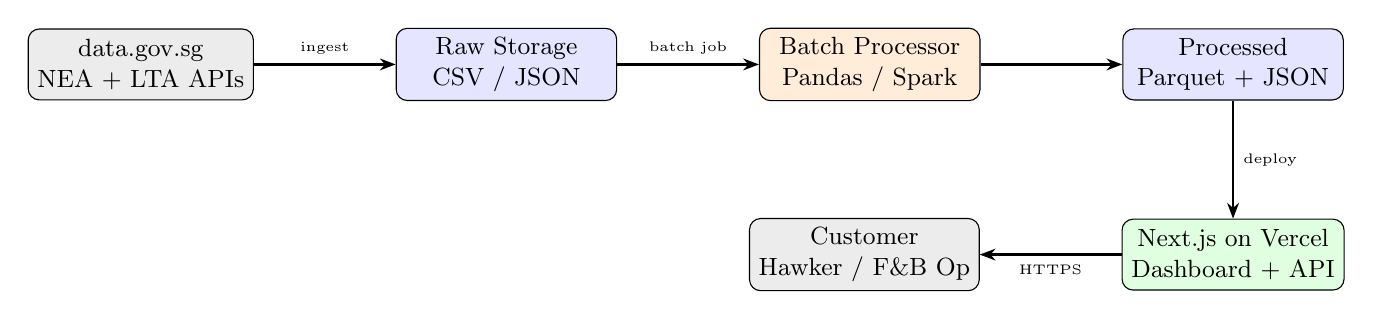
\begin{tikzpicture}[
  node distance=1.2cm and 1.8cm,
  box/.style={draw, rounded corners, minimum width=2.8cm, minimum height=0.9cm, align=center, font=\small},
  store/.style={box, fill=blue!10},
  proc/.style={box, fill=orange!15},
  deliver/.style={box, fill=green!12},
  arrow/.style={-{Stealth[length=2mm]}, thick}
]
  \node[box, fill=gray!15] (dg) {data.gov.sg\\NEA + LTA APIs};
  \node[store, right=of dg] (raw) {Raw Storage\\CSV / JSON};
  \node[proc, right=of raw] (batch) {Batch Processor\\Pandas / Spark};
  \node[store, right=of batch] (parq) {Processed\\Parquet + JSON};
  \node[deliver, below=1.5cm of parq] (vercel) {Next.js on Vercel\\Dashboard + API};
  \node[box, fill=gray!15, left=of vercel] (user) {Customer\\Hawker / F\&B Op};

  \draw[arrow] (dg) -- (raw) node[midway, above, font=\tiny] {ingest};
  \draw[arrow] (raw) -- (batch) node[midway, above, font=\tiny] {batch job};
  \draw[arrow] (batch) -- (parq);
  \draw[arrow] (parq) -- (vercel) node[midway, right, font=\tiny] {deploy};
  \draw[arrow] (vercel) -- (user) node[midway, below, font=\tiny] {HTTPS};
\end{tikzpicture}
\caption{StallPulse end-to-end architecture}
\label{fig:arch}
\end{figure}

\subsection{Scalability and Cost at 10$\times$ and 100$\times$}

\textbf{10$\times$ (500 subscribers, 250 centres):}
\begin{itemize}
  \item Migrate batch processing to Apache Spark (local $\rightarrow$ 4-node cluster).
  \item Store processed data in PostgreSQL (Neon serverless) instead of static JSON.
  \item Add Redis cache for API hot queries.
  \item Estimated infra: S\$200/month.
\end{itemize}

\textbf{100$\times$ (5,000 subscribers, 1,000+ centres):}
\begin{itemize}
  \item Stream NEA updates via Kafka; incremental scoring with Spark Structured Streaming.
  \item Data lake on S3/GCS with Parquet partitioning by planning area.
  \item CDN for static reports; API rate limiting via API gateway.
  \item Estimated infra: S\$1,500/month vs.\ S\$145,000 MRR (99\% gross margin).
\end{itemize}

%==============================================================================
\section{Repository and Deployment}
%==============================================================================

The project repository contains:
\begin{itemize}
  \item \texttt{scripts/ingest/} --- data.gov.sg ingestion scripts
  \item \texttt{scripts/process/} --- batch scoring pipeline
  \item \texttt{scripts/demand-research/} --- demand evidence collection
  \item \texttt{web/} --- Next.js delivery application
  \item \texttt{data/} --- raw and processed sample data
  \item \texttt{report/report.tex} --- this document
\end{itemize}

Deploy the web app to Vercel by pointing the project root to \texttt{web/}. See \texttt{VERCEL.md} for step-by-step instructions.

%==============================================================================
\section{Conclusion}
%==============================================================================

StallPulse demonstrates that public government data, when refined through a batch analytics pipeline and delivered via a focused SaaS product, can address a real and monetizable need. The hawker stall entrepreneur segment has clear pain (location selection under uncertainty), validated market size (36K+ establishments), and willingness to pay (S\$29--99/month) anchored against alternatives costing 100$\times$ more. Technical risks (rate limits, coarse geocoding) and business risks (trust, cold-start) are manageable with transparent sourcing and iterative model improvement.

\end{document}
